% figure to illustrate KMP match
\ifdefined\includetikz\relax \else
%\documentclass{standalone}
\documentclass{article}
\usepackage{tikz}
\usepackage{amsmath}
\usetikzlibrary{matrix,positioning}
\begin{document}
\fi

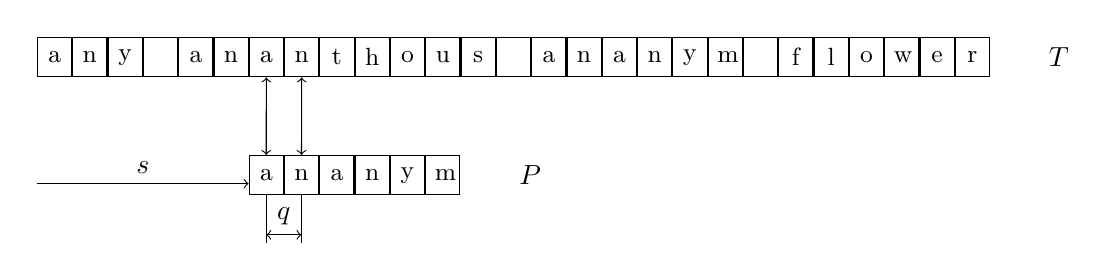
\begin{tikzpicture}[
scale=0.5,
array/.style={matrix of nodes,
              font=\small,
              minimum height=5mm, text width=2mm,
              nodes={draw, align=center, anchor=south},
              nodes in empty cells
              }]

%any ananthous ananym flower
\matrix[array] (mytext) {
a & n & y & & a & n & a & n & t & h & o & u & s & & a & n & a & n & y & m & & f & l & o & w & e & r \\};
\node[right=0.5cm of mytext] {$T$};

%ananym
\matrix[array,
  anchor=west] at ([yshift=-3cm, xshift=-0.7cm]mytext-1-7) (myptn) {
a & n & a & n & y & m \\};
\node[right=0.5cm of myptn] {$P$};

% offset s
\draw[->] ([yshift=-2.7cm]mytext-1-1.south west) -- node[above] {$s$} ([yshift=-2.7cm]mytext-1-6.south east);

% matches chars so far.
\foreach \i/\j in {7/1, 8/2} {
  \draw[<->] (mytext-1-\i.south) -- (myptn-1-\j.north);
}

% matched count q.
\draw (myptn-1-1.south) -- ++(0, -1.2cm);
\draw (myptn-1-2.south) -- ++(0, -1.2cm);
\draw[<->] ([yshift=-1cm]myptn-1-1.south) -- node[above] {$q$} ([yshift=-1cm]myptn-1-2.south);

\end{tikzpicture}

\ifdefined\includetikz\relax \else
\end{document}
\fi
